\section{SBERT Downstream Tasks}
\label{sec:sbert}

Sentence embedding is built on Siamese-style training \citep{reimers_sentence-bert_2019}. For sentence pair $(s_1,s_2)$ with embeddings $(e_1,e_2)$:
\[
\text{cos}(e_1,e_2)=\frac{e_1^\top e_2}{\|e_1\|\|e_2\|}
\]
and regression-style cosine loss:
\[
\mathcal{L}_{\text{cos}}=\left(\text{cos}(e_1,e_2)-y\right)^2
\]
with $y\in[-1,1]$ in this pipeline.

Supported downstream modes:
\begin{itemize}[leftmargin=*]
    \item \textbf{Similarity}: pairwise score between two sentences.
    \item \textbf{Search}: top-$k$ nearest neighbors over a corpus.
    \item \textbf{Cluster}: grouping embeddings (e.g., k-means).
    \item \textbf{Encode}: persistent embedding export for later retrieval.
\end{itemize}

\begin{figure}[t]
\centering
\fitfigure{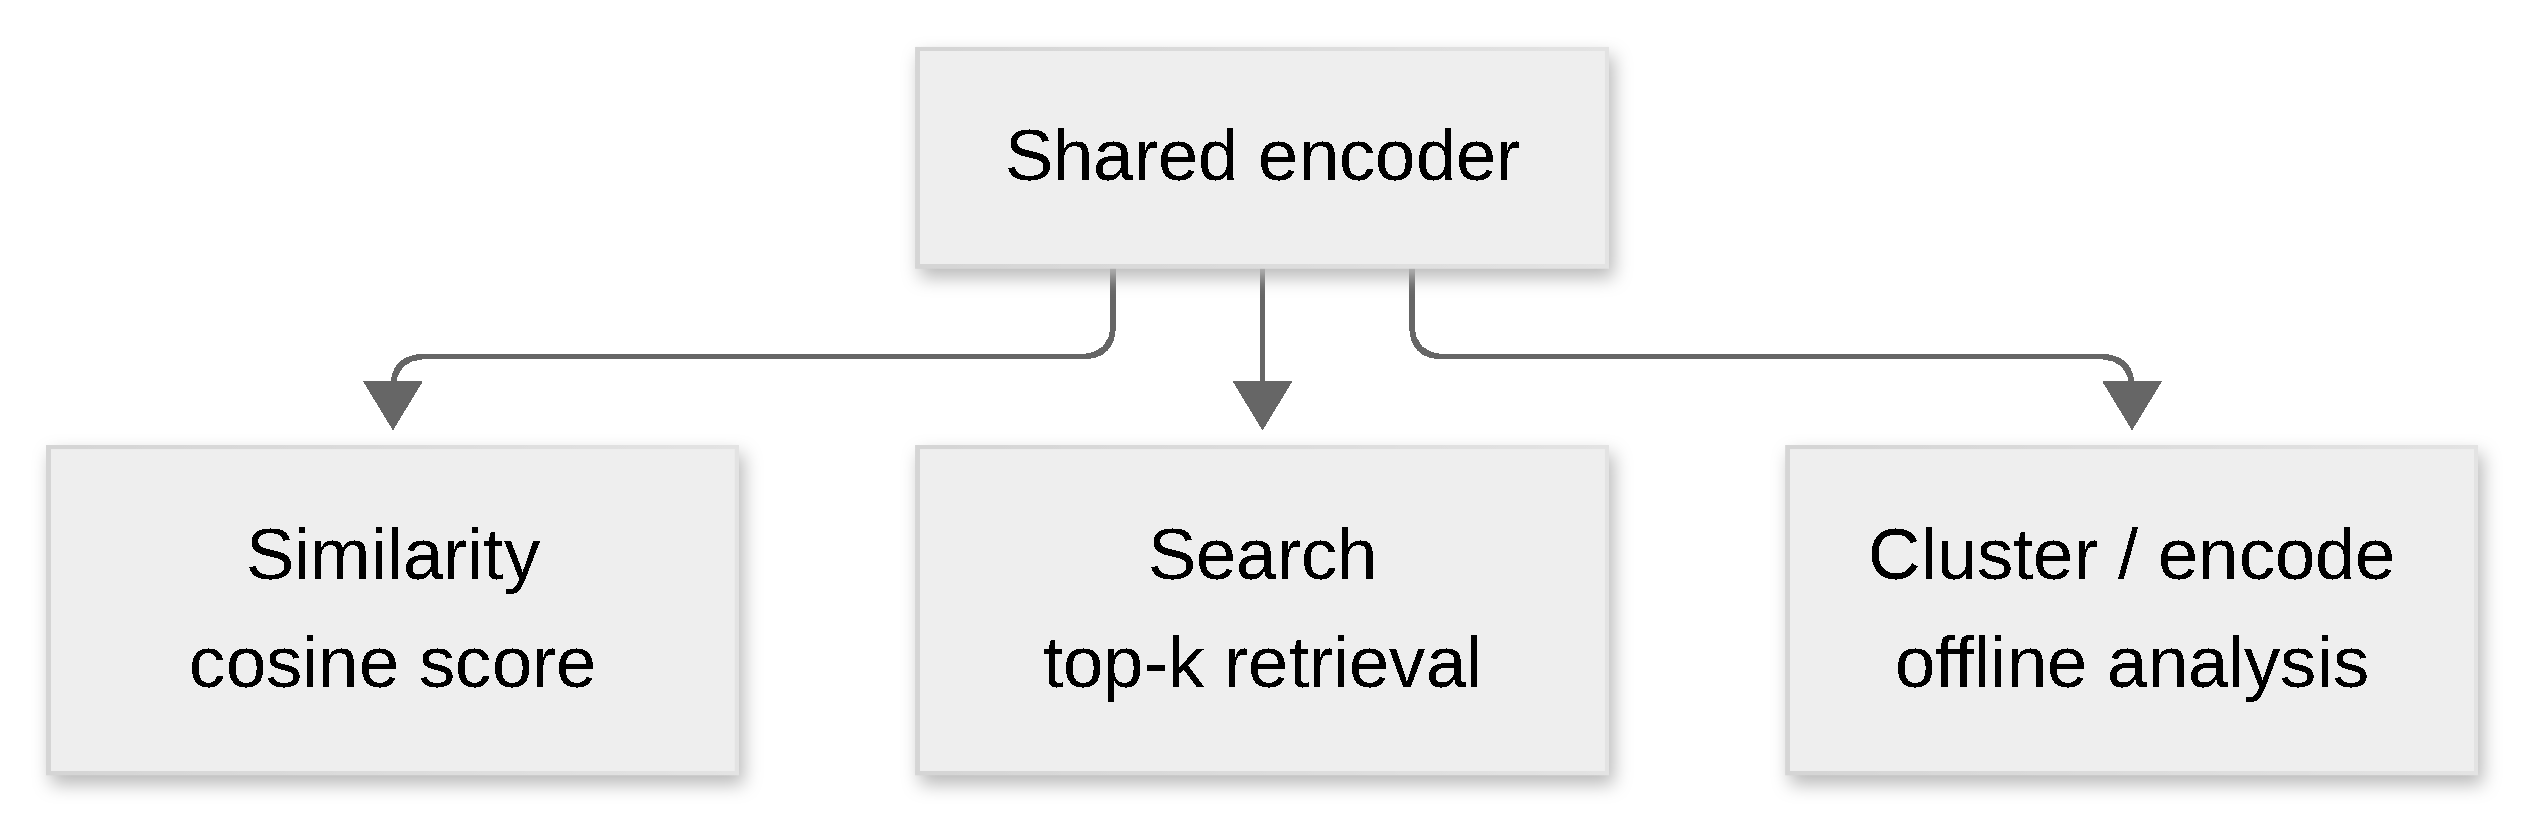
\includegraphics{figures/sbert-modes.pdf}}
\caption{SBERT workflow reuse. A single encoder supports online pair scoring, corpus retrieval, clustering, and persistent embedding export.}
\label{fig:sbert-modes}
\end{figure}

The pseudocode for the SBERT inference mode router---dispatching among similarity, search, cluster, and encode modes over a shared encoder---is deferred to Appendix~\ref{sec:annex-norm-bitnet-mod}.

